\documentclass{oblivoir}
\usepackage{amsmath,amssymb,amsthm,kotex,mdframed,paralist,kswrapfig}
\usepackage{caption, subcaption}

\newcounter{num}
\newcommand{\prob}
{\bigskip\noindent\refstepcounter{num}\textbf{문제 \arabic{num})}\par}

\newcommand{\ans}{\par{\raggedleft\textbf{답 : (\qquad\qquad\qquad\qquad\qquad\qquad)}
\par}\bigskip\bigskip}


%%%
\begin{document}
\Large

\title{승재 21 - 6학년 2학기 - 14}
\author{}
\date{\today}
\maketitle
%\tableofcontents

\newpage

다음 그림을 보고 물음에 답하세요(문제1--문제3).
\begin{figure}[h!]
    \centering
    \begin{subfigure}[b]{0.3\textwidth}
        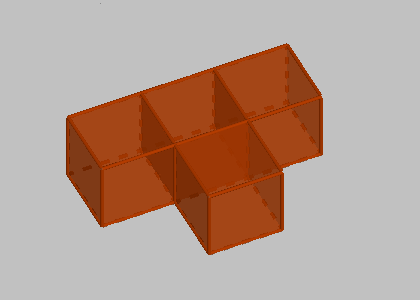
\includegraphics[width=\textwidth]{block_01}
        \caption{}
    \end{subfigure}
    ~ 
    \begin{subfigure}[b]{0.3\textwidth}
        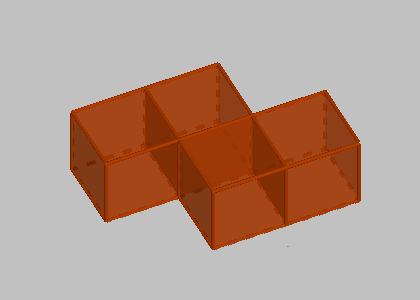
\includegraphics[width=\textwidth]{block_02}
        \caption{}
    \end{subfigure}
    ~ 
    \begin{subfigure}[b]{0.3\textwidth}
        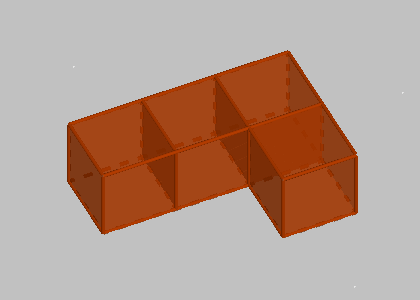
\includegraphics[width=\textwidth]{block_03}
        \caption{}
    \end{subfigure}

    \begin{subfigure}[b]{0.3\textwidth}
        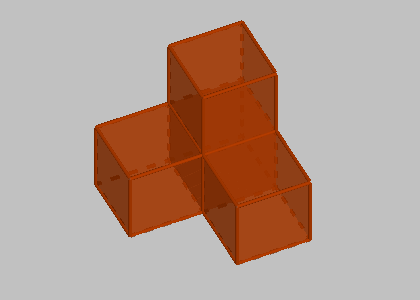
\includegraphics[width=\textwidth]{block_04}
        \caption{}
    \end{subfigure}
    ~ 
    \begin{subfigure}[b]{0.3\textwidth}
        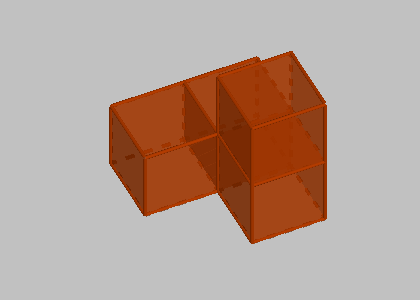
\includegraphics[width=\textwidth]{block_05}
        \caption{}
    \end{subfigure}
    ~ 
    \begin{subfigure}[b]{0.3\textwidth}
        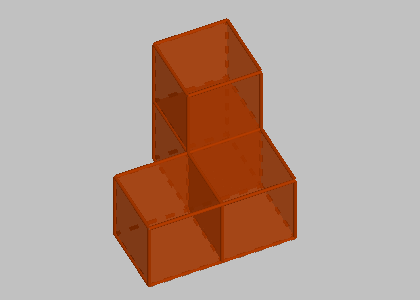
\includegraphics[width=\textwidth]{block_06}
        \caption{}
    \end{subfigure}
\end{figure}

%
\stepcounter{num}
\kswrapfig[Pos=r]{01}{
\textbf{문제 1)}\\
오른쪽 모양을 만들기 위해 필요한 쌓기나무 모양 2가지는 어느 것인지 기호를 쓰세요.
\ans
}

%
\stepcounter{num}
\kswrapfig[Pos=r]{02}{
\textbf{문제 2)}\\
오른쪽 모양을 만들기 위해 필요한 쌓기나무 모양 2가지는 어느 것인지 기호를 쓰세요.
\ans
}

%
\stepcounter{num}
\kswrapfig[Pos=r]{03}{
\textbf{문제 3)}\\
오른쪽 모양을 만들기 위해 필요한 쌓기나무 모양 2가지는 어느 것인지 기호를 쓰세요.
\ans
}

\newpage

%
\prob
쌓기나무로 쌓은 모양을 위, 앞, 옆에서 본 그림입니다.
모두 몇 가지를 만들 수 있습니까?
\begin{figure}[h]
\centering
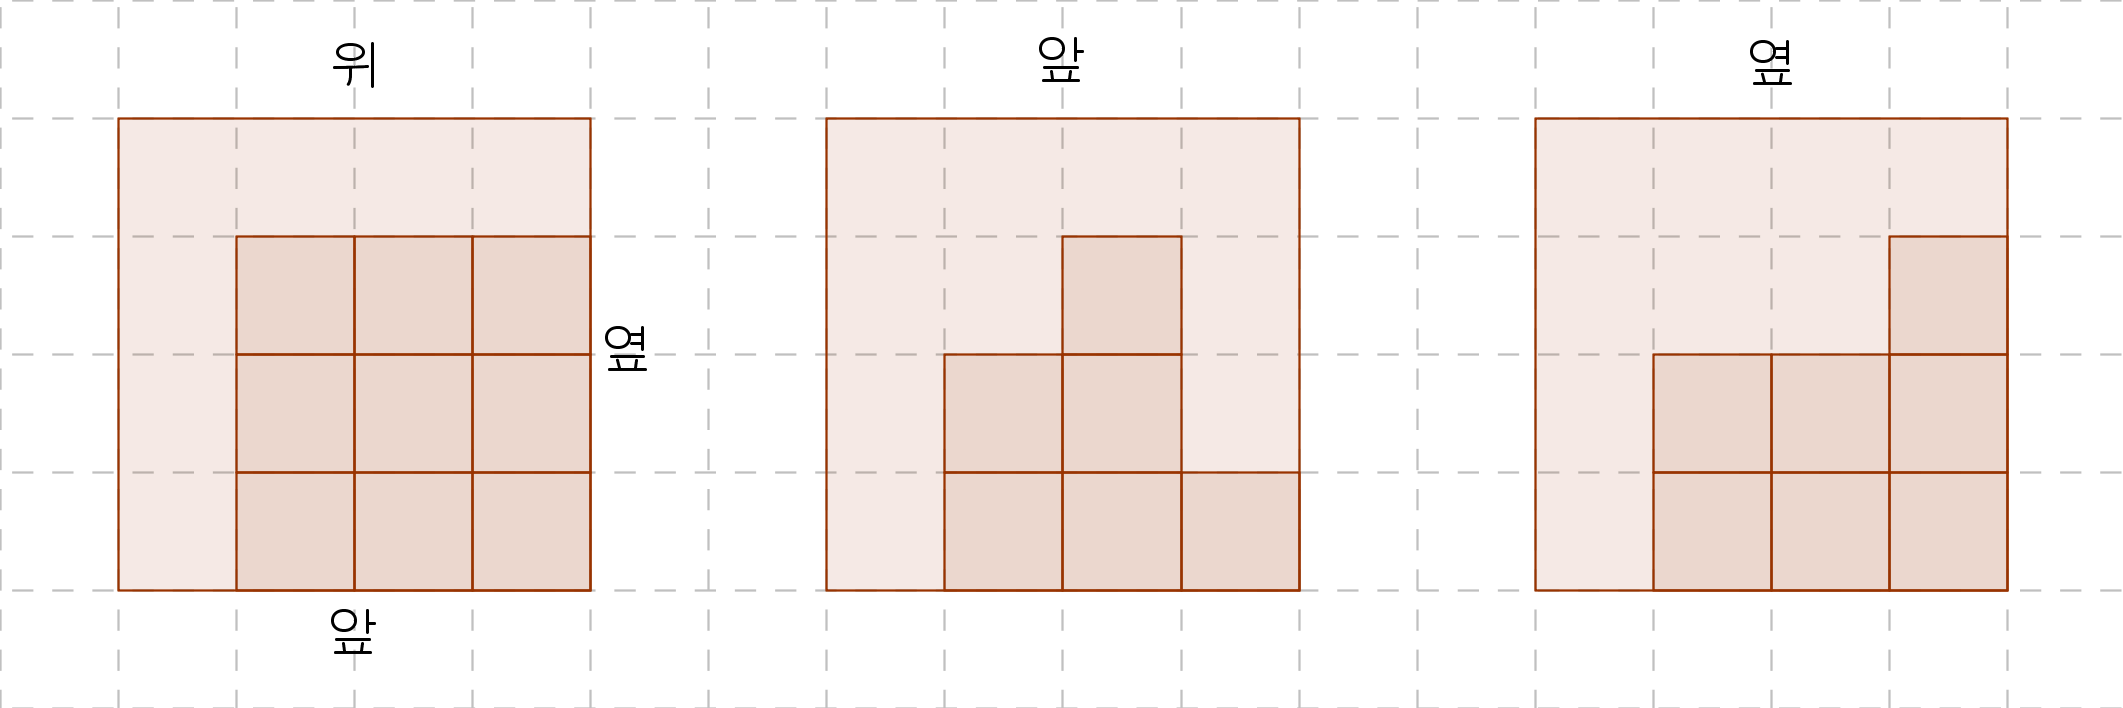
\includegraphics[width=\textwidth]{04}
\end{figure}
\ans

%
\prob
쌓기나무로 쌓은 모양을 위, 앞, 옆에서 본 그림입니다.
모두 몇 가지를 만들 수 있습니까?
\begin{figure}[h]
\centering
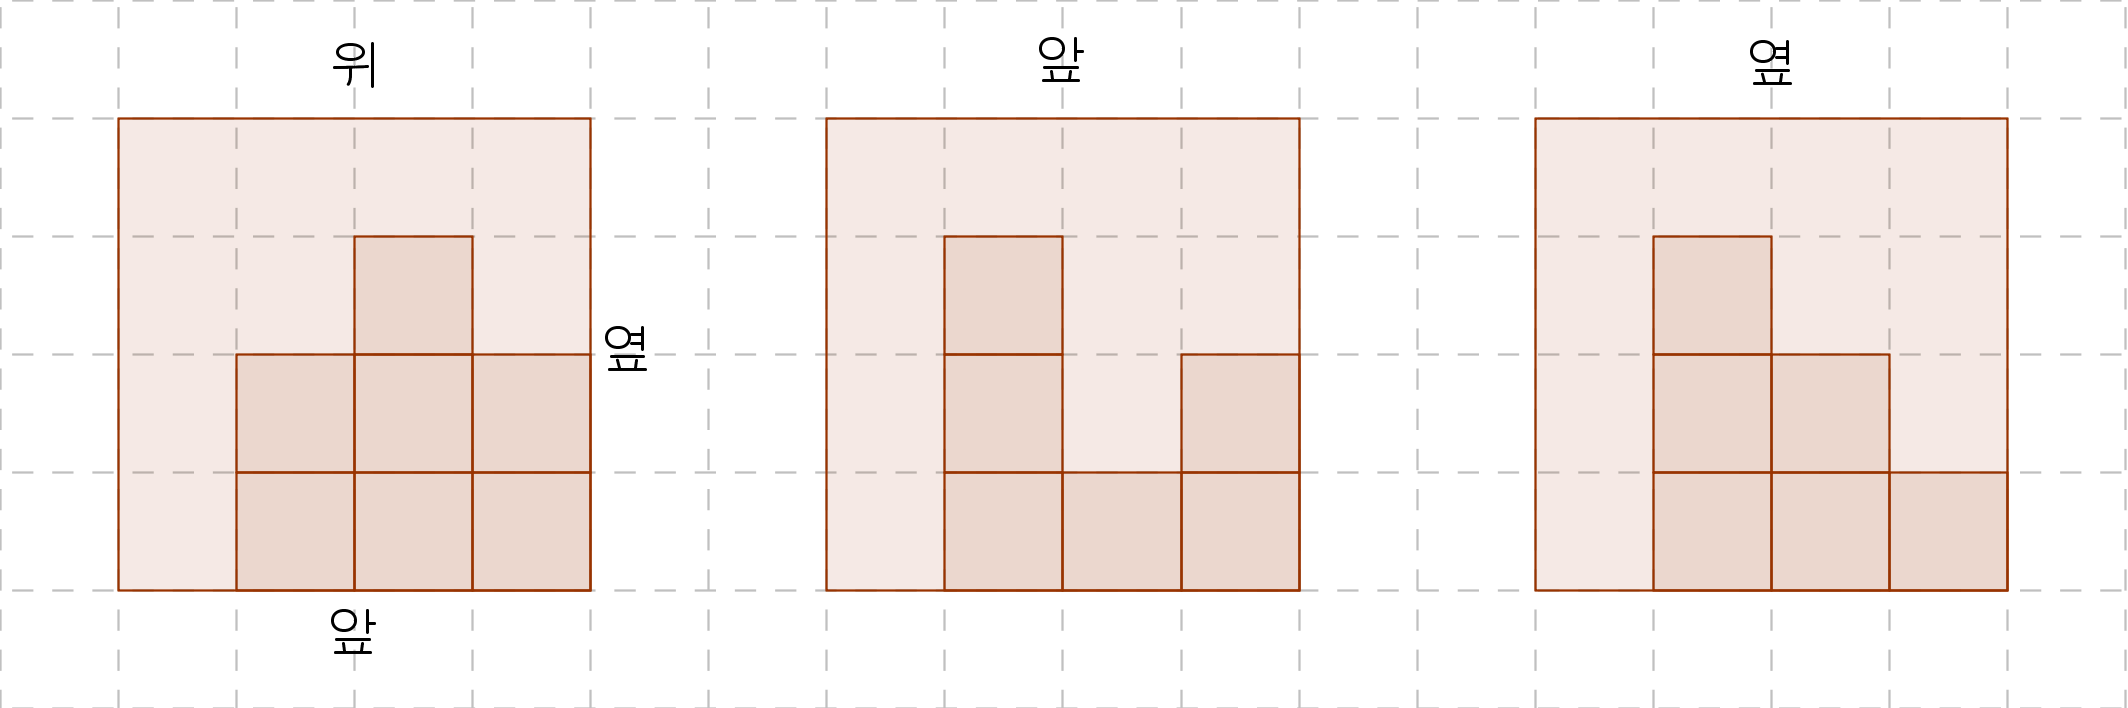
\includegraphics[width=\textwidth]{05}
\end{figure}
\ans

\newpage


%
\prob
아래 그림과 같이 27개의 쌓기나무로 정육면체를 만든 후 모든 바깥쪽 면을 색칠하고 다시 각각 떼어 놓았더니 색이 하나도 칠해지지 않은 쌓기나무가 1개였습니다.
이와 같이 쌓기나무로 정육면체를 쌓은 후 바깥쪽 면을 색칠하고 각각 떼어 놓았을 때, 색이 두 면만 칠해진 쌓기나무가 48개가 되도록 하려고 합니다.
쌓기나무 몇 개로 정육면체를 쌓아야 합니까?

\begin{figure}[h!]
\centering
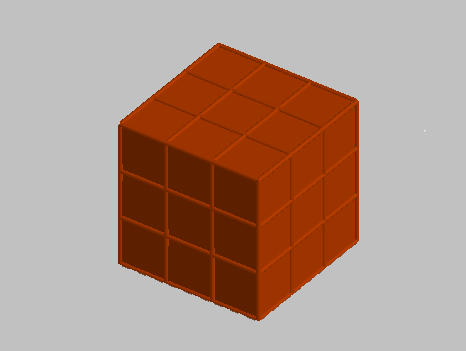
\includegraphics[width=0.5\textwidth]{06}
\end{figure}
\ans

\newpage

%
\prob
아래 그림과 같이 겹쳐진 두 원 (가)와 (나)의 넓이의 비는 3:2 입니다.
겹쳐진 부분의 넓이가 (가)의 넓이의 \(\frac13\)라 할 때, 겹쳐진 부분의 넓이는 원 (나)의 넓이의 몇 \%입니까?
\begin{figure}[h!]
\centering
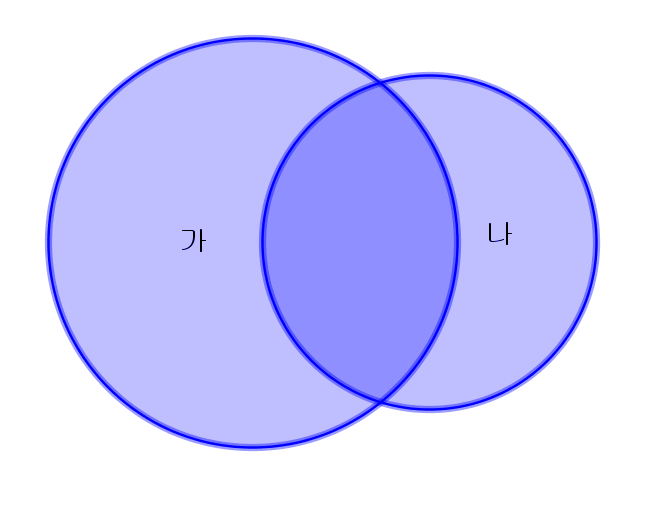
\includegraphics[width=0.5\textwidth]{07}
\end{figure}
\ans

%
\prob
아래 그림과 같이 겹쳐진 두 원 (가)와 (나)의 넓이의 비는 6:5 입니다.
겹쳐진 부분의 넓이가 (가)의 넓이의 \(\frac16\)라 할 때, 겹쳐진 부분의 넓이는 원 (나)의 넓이의 몇 \%입니까?
\begin{figure}[h!]
\centering
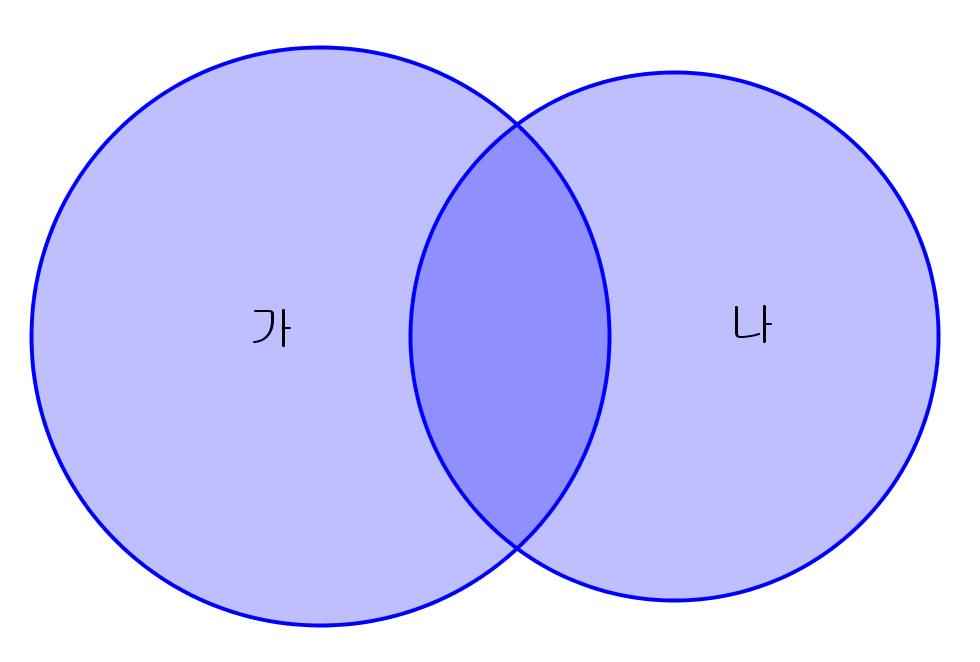
\includegraphics[width=0.5\textwidth]{08}
\end{figure}
\ans

\newpage
%
\prob
아래 그림과 같이 겹쳐진 두 원 (가)와 (나)의 넓이의 비는 15:24 입니다.
겹쳐진 부분의 넓이가 (가)의 넓이의 \(\frac35\)라 할 때, 겹쳐진 부분의 넓이는 원 (나)의 넓이의 몇 \%입니까?
\begin{figure}[h!]
\centering
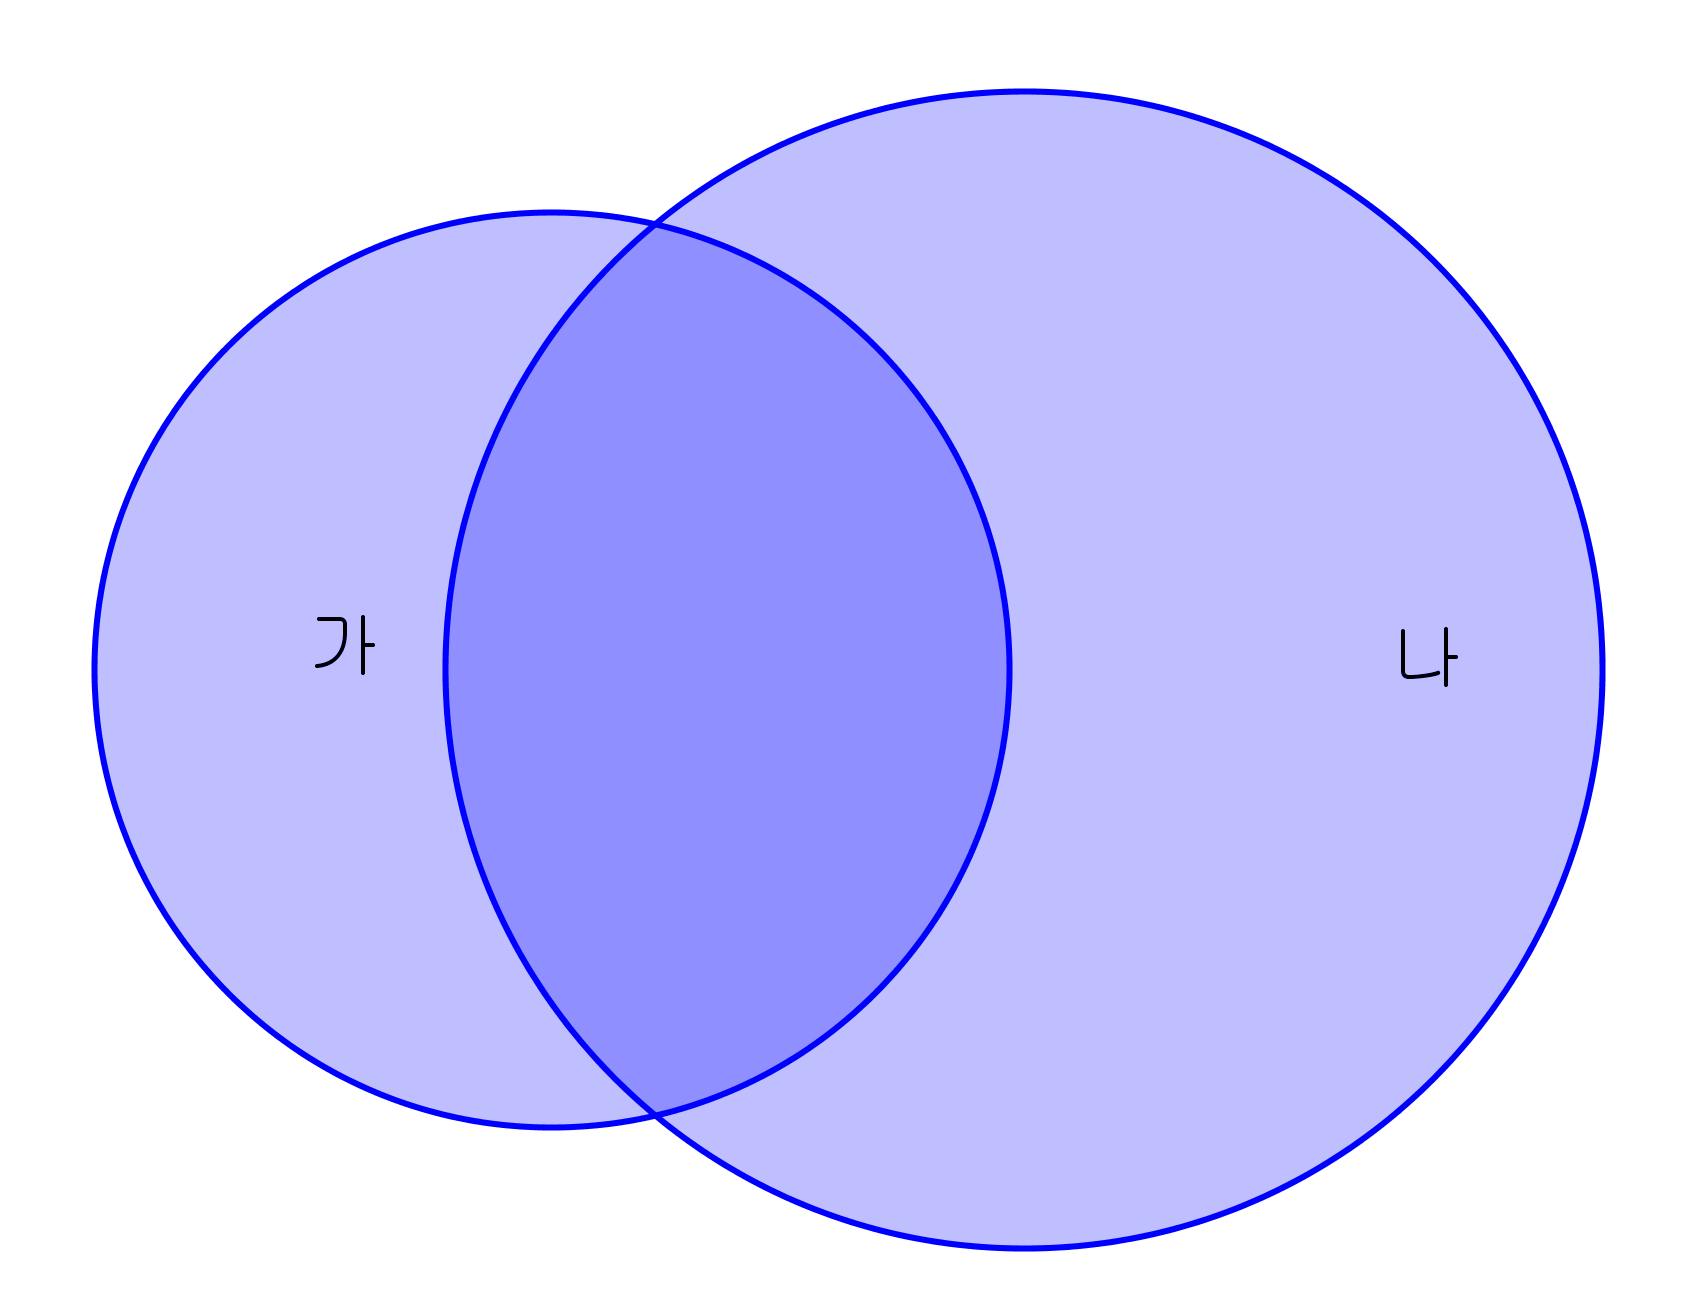
\includegraphics[width=0.5\textwidth]{09}
\end{figure}
\ans

%
\prob
아래 그림과 같이 겹쳐진 두 원 (가)와 (나)의 넓이의 비는 27:20 입니다.
겹쳐진 부분의 넓이가 \(18\)cm\(^2\)이고, 이것은 (가)의 넓이의 \(\frac29\)입니다.
원 (나)의 넓이를 구하세요.
%라 할 때, 겹쳐진 부분의 넓이는 원 (나)의 넓이의 몇 \%입니까?
\begin{figure}[h!]
\centering
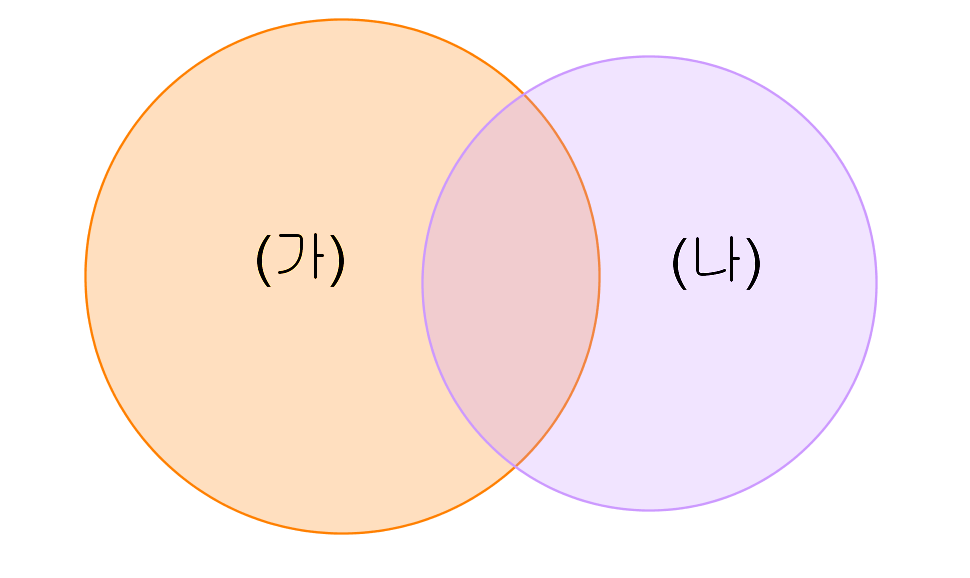
\includegraphics[width=0.5\textwidth]{10}
\end{figure}
\ans

\newpage

%
\prob
아래 그림과 같이 직사각형 (가)와 (나)가 겹쳐져 있습니다.
겹쳐진 부분의 넓이는 (가)의 넓이의 \(30\%\)이고, (나)의 넓이의 \(\frac14\)입니다.
직사각형 (가)와 (나)의 넓이의 비를 가장 간단한 자연수의 비로 나타내세요.
\begin{figure}[h!]
\centering
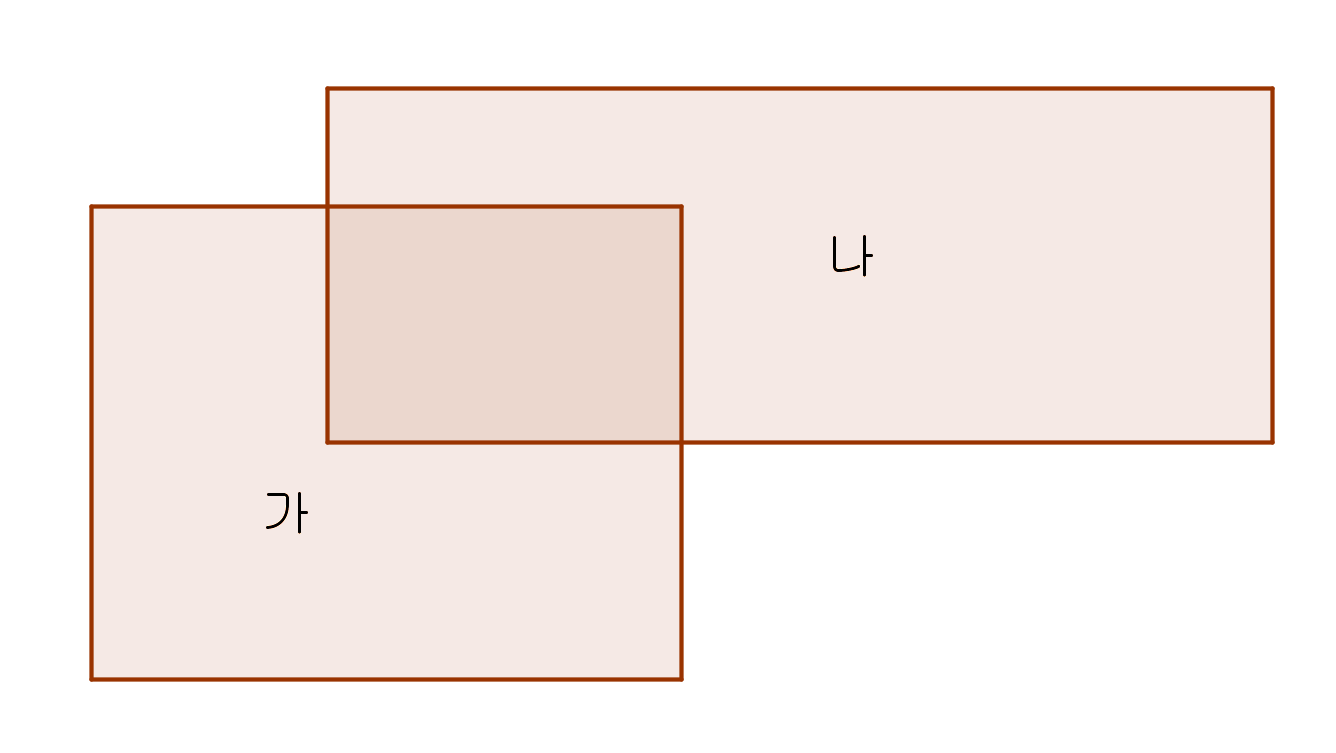
\includegraphics[width=0.5\textwidth]{11}
\end{figure}
\ans

%
\prob
아래 그림과 같이 겹쳐진 두 직사각형 (가)와 (나)의 넓이의 비가 21:25 입니다.
겹쳐진 부분의 넓이는 (가)의 넓이의 \(\frac27\)일 때, 겹쳐진 부분의 넓이는 직사각형 (나)의 넓이의 몇 \%입니까?
\begin{figure}[h!]
\centering
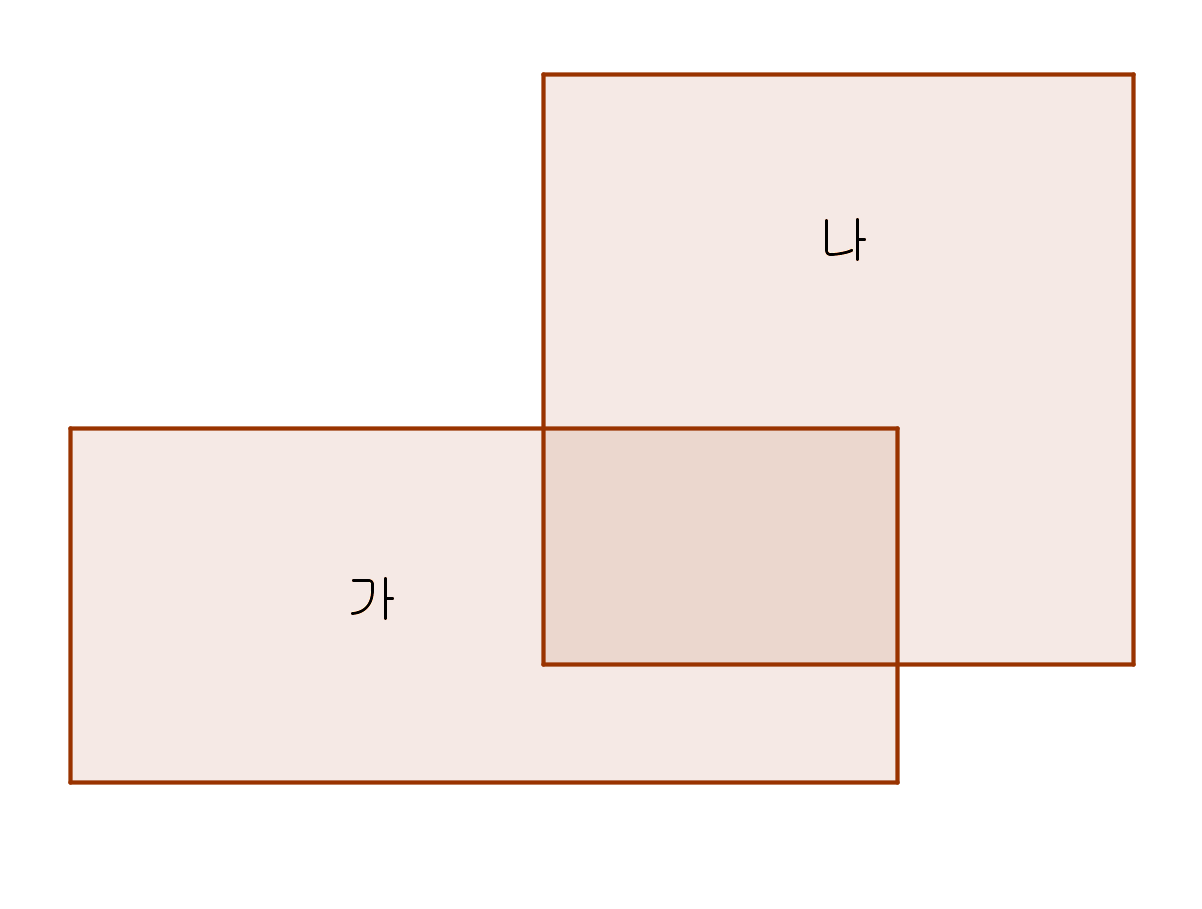
\includegraphics[width=0.5\textwidth]{12}
\end{figure}
\ans

\newpage

%
\prob
아래 그림과 같이 두 직사각형 (가)와 (나)가 겹쳐져 있습니다.
겹쳐진 부분의 넓이는 (가)의 넓이의 \(\frac4{15}\)이고, (나)의 넓이의 20\%입니다.
직사각형 (가)와 (나)의 넓이의 합이 cm\(84^2\)일 때, 직사각형 (나)의 넓이를 구하세요.
\begin{figure}[h!]
\centering
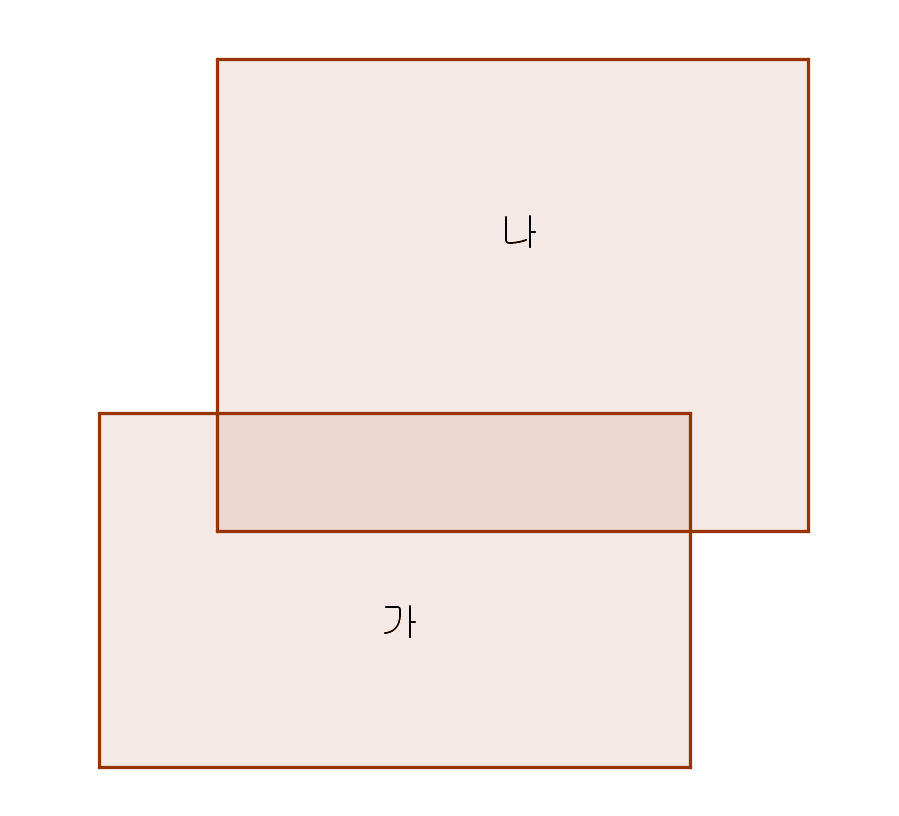
\includegraphics[width=0.5\textwidth]{13}
\end{figure}
\ans

\newpage

%
\prob
어머니께서 사오신 고구마, 감자, 당근의 무게의 합은 \(6\)kg입니다.
고구마의 무게가 감자의 무게의 \(\frac37\)이고, 감자의 무게는 당근의 무게의 \(1\frac25\)일 때, 고구마의 무게는 몇 kg 몇 g 입니까?
\ans

%
\prob
어머니께서 사오신 고구마, 감자, 당근의 무게의 합은 \(5\)kg입니다.
고구마의 무게가 감자의 무게의 \(\frac13\)이고, 감자의 무게는 당근의 무게의 \(1\frac13\)일 때, 고구마의 무게는 몇 kg 몇 g 입니까?
\ans

\newpage

%
\prob
학교 앞 문구점에서 강아지 인형의 가격을 20\% 올려 6000원에 판매하고 있습니다.
강아지 인형의 가격이 오르기 전과 오른 후의 비를 가장 간단한 자연수의 비로 나타내세요.
\ans

%
\prob
학교 앞 문구점에서 강아지 인형의 가격을 15\% 올려 6900원에 판매하고 있습니다.
강아지 인형의 가격이 오르기 전과 오른 후의 비를 가장 간단한 자연수의 비로 나타내세요.
\ans

%
\prob
학교 앞 문구점에서 고양이 인형의 가격을 25\% 할인해 8800원에 판매하고 있습니다.
고양이 인형의 가격이 할인되기 전과 할인된 후의 비를 가장 간단한 자연수의 비로 나타내세요.
\ans

%
\prob
학교 앞 문구점에서 고양이 인형의 가격을 8\% 할인해 6900원에 판매하고 있습니다.
고양이 인형의 가격이 할인되기 전과 할인된 후의 비를 가장 간단한 자연수의 비로 나타내세요.
\ans

\newpage

%
\prob
두 숫자 (가)와 (나)에 대해서 (가)의 \(1\frac45\)가 (나)의 \(20\%\)와 같다고 합니다.
이 때, (가)와 (나)의 비를 가장 간단한 자연수의 비로 나타내세요.
\ans

%
\prob
두 숫자 (가)와 (나)에 대해서 (가)의 \(\frac19\)가 (나)의 \(30\%\)와 같다고 합니다.
이 때, (가)와 (나)의 비를 가장 간단한 자연수의 비로 나타내세요.
\ans

%
\prob
두 상품 (가)와 (나)가 있습니다.
(가) 상품 정가의 10\%를 할인한 금액과 (나) 상품 정가의 0.1를 인상한 금액이 같다고 합니다.
(가) 상품과 (나) 상품의 정가를 가장 간단한 자연수의 비로 나타내세요.
\ans

%
\prob
두 상품 (가)와 (나)가 있습니다.
(가) 상품 정가의 5\%를 할인한 금액과 (나) 상품 정가의 0.05를 인상한 금액이 같다고 합니다.
(가) 상품과 (나) 상품의 정가를 가장 간단한 자연수의 비로 나타내세요.
\ans

%
\prob
사랑이네 학교 학생들이 좋아하는 계절을 조사하여 나타낸 띠그래프입니다.
봄을 좋아하는 학생은 99명이고, 봄을 좋아하는 학생 수는 여름을 좋아하는 학생 수의 75\%일 때, 사랑이네 학교 학생 수는 모두 몇 명입니까?
\begin{figure}[h!]
\centering
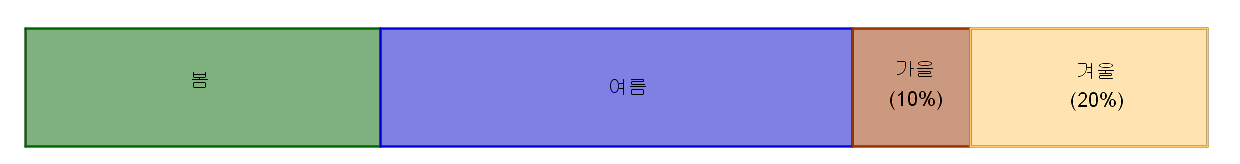
\includegraphics[width=0.9\textwidth]{25}
\end{figure}
\ans

%
\prob
사랑이네 학교 학생들이 좋아하는 계절을 조사하여 나타낸 띠그래프입니다.
봄을 좋아하는 학생은 30명이고, 봄을 좋아하는 학생 수는 여름을 좋아하는 학생 수의 40\%일 때, 사랑이네 학교 학생 수는 모두 몇 명입니까?
\begin{figure}[h!]
\centering
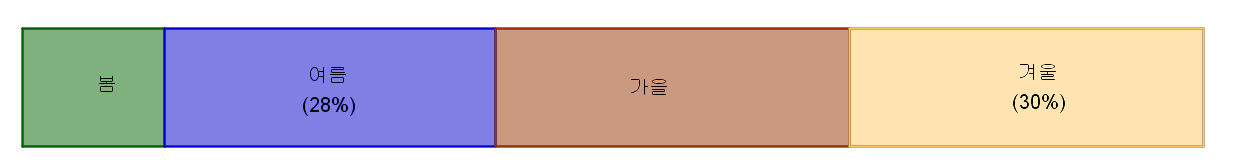
\includegraphics[width=0.9\textwidth]{26}
\end{figure}
\ans

\newpage
%
\prob
어떤 초등학교의 학생들이 좋아하는 계절을 조사하여 나타낸 띠그래프입니다.
가을을 좋아하는 학생은 364명이고, 가을을 좋아하는 학생 수는 겨울을 좋아하는 학생 수의 70\%일 때, 이 학교의 학생 수는 모두 몇 명입니까?
\begin{figure}[h!]
\centering
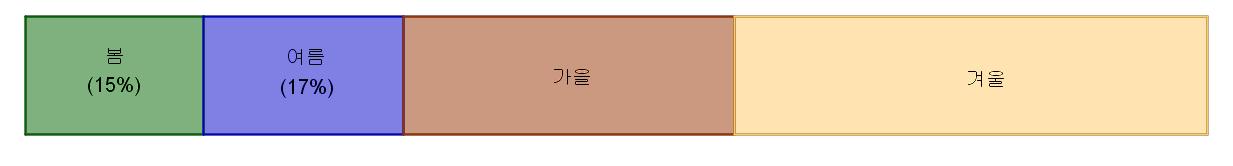
\includegraphics[width=0.9\textwidth]{27}
\end{figure}
\ans

\newpage

%
\prob
아래 그림에서 선분 AB와 선분 BD의 길이의 비는 5:13이고 선분 AC와 선분 CD의 길이의 비는 5:4입니다.
선분 BC의 길이가 15cm일 때, 전체 선분의 길이를 구하세요.

\begin{figure}[h!]
\centering
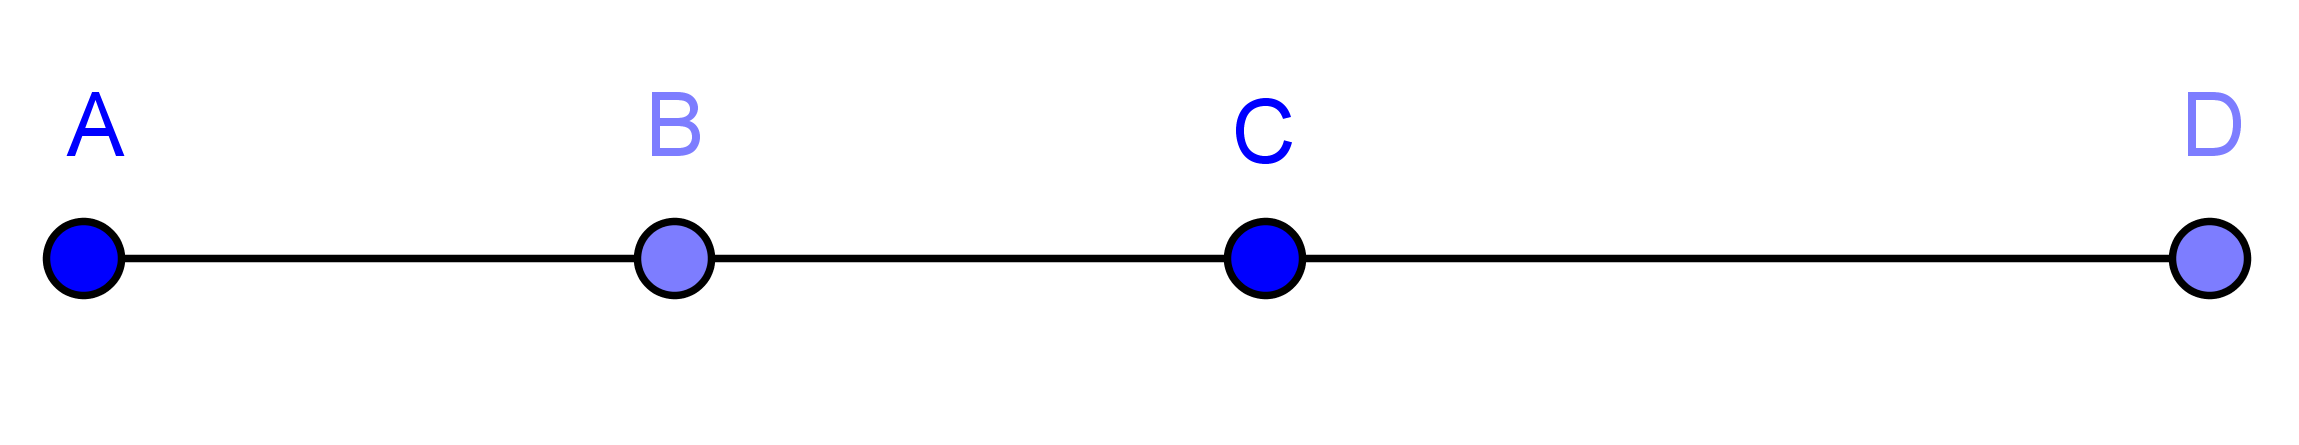
\includegraphics[width=0.5\textwidth]{28}
\end{figure}
\ans

%
\prob
아래 그림에서 선분 AB와 선분 BD의 길이의 비는 2:7이고 선분 AC와 선분 CD의 길이의 비는 5:1입니다.
선분 BC의 길이가 5.5cm일 때, 전체 선분의 길이를 구하세요.
\begin{figure}[h!]
\centering
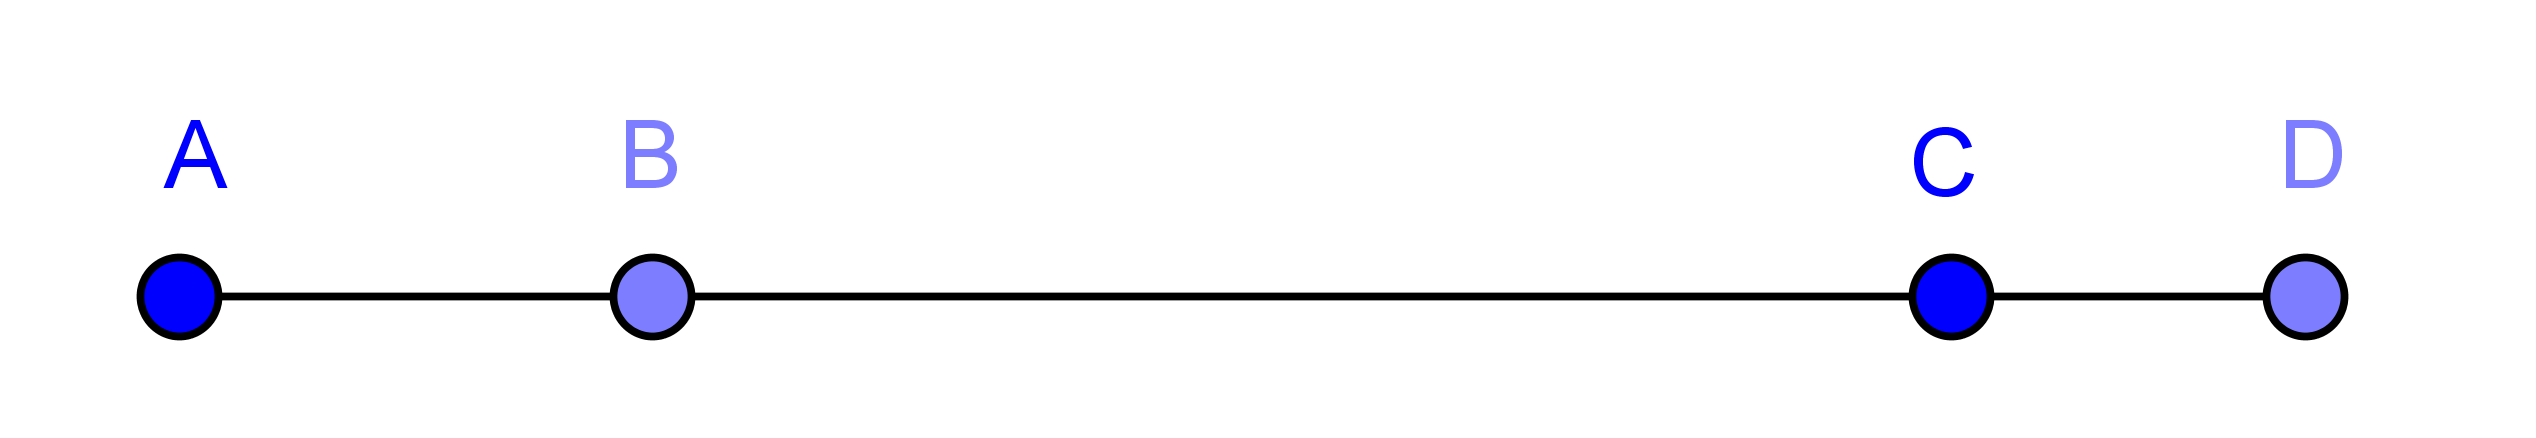
\includegraphics[width=0.5\textwidth]{29}
\end{figure}
\ans

\newpage

%
\prob
어떤 일을 하는 데 민희가 혼자 일을 하면 6시간이 걸리고, 유리가 혼자 일을 하면 9시간이 걸립니다.
이 일을 민희와 유리가 함께 일을 한다면 일을 마치는 데 몇 시간 몇 분이 걸립니까?

\ans

%
\prob
어떤 일을 하는 데 6학년 학생이 혼자 일을 하면 4시간이 걸리고, 3학년 학생이 혼자 일을 하면 6시간이 걸리는 일이 있습니다.
6학년 학생 한 명과 3학년 학생 두 명이 같이 일을 하면 일을 마치는 데 몇 시간 몇 분이 걸립니까?
\ans
\end{document}